\section{Evaluation of CEGAR}

\subsection{Comparison to Symbolic Execution CPA without CEGAR}
Evaluation shows the great boost CEGAR provides to the \symbolicExecutionCPA. 
Table~\ref{tab:cegarBenefits} shows the results of the \symbolicExecutionCPA\ without CEGAR using the subset less-or-equal operator and $\cpaMerge^{sep}$ (SymEx w/o CEGAR), in comparison to the \symbolicExecutionCPA\ using CEGAR with refinement based on CEGAR for explicit-state model checking (SymEx w/ CEGAR, Sec.~\ref{sec:assignmentRefinement}).
\emph{Program errors} are errors in the execution of \cpaChecker, in this case a parsing error of a file for both analysis and an exception due to a failure of the SMT solver in the analysis without CEGAR and one due to a division by zero in the analysis with CEGAR.
The increase in correctly handled tasks \emph{without} a safety violation (in the table row ''correct negatives'') by a factor of more then 10
and the decrease in timeouts by more then 40\% are the most notable improvements by using CEGAR.
On the contrary, the number of found safety violations decreases by 222 tasks,
since the lazy approach of CEGAR has a problem with programs consisting of a lot of assumptions leading to an error in dependence of many variables.

\begin{table}[t]
\centering
\begin{tabular}{|r|c|c|c|}
\hline
    & SymEx w/o CEGAR & SymEx w/ CEGAR & Overall \\ \hline
correct results & 761 (18.60\%) & 2078 (50.78\%) & 4092 \\ \hline
\resultFalse, correct & 598 (50.63\%) & 376 (31.83\%) & 1181 \\ \hline
\resultTrue, correct & 163 (5.599\%) & 1702 (58.47\%) & 2911 \\ \hline
unique \resultFalse, correct & 323 & 101 & \\ \hline
unique \resultTrue, correct & 84 & 1623 & \\ \hline
\resultFalse, incorrect & 44 & 83 & \\ \hline
unique \resultFalse, incorrect & 4 & 43 & \\ \hline
\resultTrue, incorrect & 0 & 1 & \\ \hline
program errors & 2 & 2 & \\ \hline % exception because of / 0, parsing error at both
%timeouts & 3275 & 1927 & \\ \hline
resource errors & 3285 & 1928 & \\ \hline % includes timeouts + StackOverflowException
\end{tabular}
\caption{Results of benchmark runs of the \symbolicExecutionCPA\ without CEGAR and with CEGAR}
\label{tab:cegarBenefits}
\end{table}

\begin{figure}
\begin{subfigure}[b]{.3\textwidth}
\centering
\begin{tikzpicture}[->,>=stealth, mynode/.style={rectangle, draw, minimum height=0.5cm, minimum width=0.8cm}, every node/.style={font=\small}]

\node[mynode] (0) {$\varnothing$};
\node[mynode] (1) [below = 0.6cm of 0] {$\varnothing$};
\node[mynode] (2) [below = 0.6cm of 1, draw=red, very thick] {$\varnothing$};

\path
  (0) edge node [left] {\textbf{a $\assign$ 2, b $\assign$ 2, ..., z $\assign$ 2}} (1)
  (1) edge node [left] {$\mathbf{[a == 1]}$} (2)
;
\end{tikzpicture}
\caption{First iteration, tracking no variables}
\label{fig:cegarFailsEx:first}
\end{subfigure}%
\hfill
\begin{subfigure}[b]{.3\textwidth}
\centering
\begin{tikzpicture}[->,>=stealth, mynode/.style={rectangle, draw, minimum height=0.5cm, minimum width=0.8cm}, every node/.style={font=\small}]

\node[mynode] (0) {$\varnothing$};
\node[mynode] (1) [below = 0.6cm of 0] {$\{ a \rightarrow 2 \}$};
\node[mynode] (2) [below = 0.6cm of 1] {$\{ a \rightarrow 2 \}$};
\node[mynode] (3) [below = 0.6cm of 2, draw=red, very thick] {$\{ a \rightarrow 2 \}$};

\path
  (0) edge node [left] {\textbf{a $\assign$ 2, ..., z $\assign$ 2}} (1)
  (1) edge node [left] {$\mathbf{[!(a == 1)]}$} (2)
  (2) edge node [left] {$\mathbf{[b == 1]}$} (3)
;
\end{tikzpicture}
\caption{Second iteration, tracking variable $a$}
\label{fig:cegarFailsEx:second}
\end{subfigure}%
\hfill
\begin{subfigure}[b]{.3\textwidth}
\centering
\begin{tikzpicture}[->,>=stealth, mynode/.style={rectangle, draw, minimum height=0.5cm, minimum width=0.8cm}, every node/.style={font=\small}]

\node[mynode] (0) {$\varnothing$};
\node[mynode] (1) [below = 0.6cm of 0] {$\{ a \rightarrow 2, b \rightarrow 2 \}$};
\node[mynode] (2) [below = 0.6cm of 1] {$\{ a \rightarrow 2, b \rightarrow 2 \}$};
\node[mynode] (3) [below = 0.6cm of 2] {$\{ a \rightarrow 2, b \rightarrow 2 \}$};
\node[mynode] (4) [below = 0.6cm of 3, draw=red, very thick] {$\{ a \rightarrow 2, b \rightarrow 2 \}$};

\path
  (0) edge node [left] {\textbf{a $\assign$ 2, ..., z $\assign$ 2}} (1)
  (1) edge node [left] {$\mathbf{[!(a == 1)]}$} (2)
  (2) edge node [left] {$\mathbf{[!(b == 1)]}$} (3)
  (3) edge node [left] {$\mathbf{[c == 1]}$} (4)
;
\end{tikzpicture}
\caption{Third iteration, tracking variables $a$ and $b$}
\label{fig:cegarFailsEx:third}
\end{subfigure}%
\vspace{1cm}
\begin{subfigure}[b]{.48\textwidth}
\begin{tikzpicture}[->,>=stealth, mynode/.style={circle, draw, minimum size=0.5cm}, every node/.style={font=\small}]

\node[mynode] (0) {0};
\node[mynode] (1) [below = 0.6cm of 0] {1};
\node[mynode] (l2) [below left = 0.7cm and 0.8cm of 1] {2};
\node[mynode] (r2) [below right = 0.7cm and 0.8cm of 1, draw=red, very thick] {3};
\node[mynode] (ll3) [below left = 0.7cm and 0.6cm of l2] {4};
\node[mynode] (lr3) [below right = 0.7cm and 0.6cm of l2, draw=red, very thick] {5};
\node[mynode] (llr4) [below right = 0.7cm and 0.4cm of ll3, draw=red, very thick] {6};
\node[mynode] (lll6) [below left = 2cm and 0.4cm of ll3] {7};
\node[mynode] (lllr6) [below right = 0.7cm and 0.3cm of lll6, draw=red, very thick] {9};
\node[mynode] (llll6) [below left = 0.7cm and 0.3cm of lll6] {8};

\path
  (0) edge node [left] {\textbf{a $\assign$ 2, b $\assign$ 2, ... z $\assign$ 2}} (1)
  (1) edge node [left, pos=0.3] {$\mathbf{[!(a == 1)]}$} (l2)
  (1) edge node [right, pos=0.3] {$\mathbf{[a == 1]}$} (r2)
  (l2) edge node [left, pos=0.3] {$\mathbf{[!(b == 1)]}$} (ll3)
  (l2) edge node [right, pos=0.3] {$\mathbf{[b == 1]}$} (lr3)
  (ll3) edge node [right, pos=0.3] {$\mathbf{[c == 1]}$} (llr4)
  (ll3) edge [dashed] (lll6)
  (lll6) edge node [right, pos=0.5] {$\mathbf{[z == 2]}$} (lllr6)
  (lll6) edge node [left, pos=0.5] {$\mathbf{[!(z == 2)]}$} (llll6)
;
\end{tikzpicture}
\caption{CFA}
\label{fig:cegarFailsEx:cfa}
\end{subfigure}%
\hfill
\begin{subfigure}[b]{.48\textwidth}
\centering
\begin{tikzpicture}[->,>=stealth, mynode/.style={rectangle, draw, minimum height=0.5cm, minimum width=0.8cm}, every node/.style={font=\small}]

\node[mynode] (0) {$\varnothing$};
\node[mynode] (1) [below = 0.6cm of 0] {$\{ a \rightarrow 2, b \rightarrow 2, ..., z \rightarrow 2 \}$};
\node[mynode] (2) [below = 0.6cm of 1] {$\{ a \rightarrow 2, b \rightarrow 2, ..., z \rightarrow 2 \}$};
\node[mynode] (3) [below = 0.6cm of 2 ] {$\{ a \rightarrow 2, b \rightarrow 2, ..., z \rightarrow 2 \}$};
\node[mynode] (4) [below = 2cm of 3] {$\{ a \rightarrow 2, b \rightarrow 2, ..., z \rightarrow 2 \}$};
\node[mynode] (5) [below = 0.6cm of 4, draw=red, very thick] {$\{ a \rightarrow 2, b \rightarrow 2, ..., z \rightarrow 2 \}$};

\path
  (0) edge node [left] {\textbf{a $\assign$ 2, ..., z $\assign$ 2}} (1)
  (1) edge node [left] {$\mathbf{[!(a == 1)]}$} (2)
  (2) edge node [left] {$\mathbf{[!(b == 1)]}$} (3)
  (3) edge [dashed] (4)
  (4) edge node [left] {$\mathbf{z == 2}$} (5)
;
\end{tikzpicture}
\caption{Last iteration tracking all program variables. Also equals the run of eager analysis}
\label{fig:cegarFailsEx:eager}
\end{subfigure}
%\caption{CFA representing an example program CEGAR performs worse for then eager analysis.}
%\label{fig:cegarFails}\\
\caption{A CFA representing a program CEGAR performs worse for then eager analysis and the first three
and last one iteration of analysis using CEGAR. The last iteration also equals the eager analysis.}
\label{fig:cegarFailsEx}
\end{figure}

Figure~\ref{fig:cegarFailsEx:cfa} shows a CFA representing one such program. The highlighted nodes are error locations.
Although only the last one of them is really reachable as all program variables are initialised with the concrete value $2$ at the beginning of the program,
the CEGAR algorithm visits one after the other, always refining the precision to track only one additional variable and then restarting
from the beginning of the program, since all variable assignments happen there.
The first three iterations of this procedure are shown in Figures~\ref{fig:cegarFailsEx:first} -- \ref{fig:cegarFailsEx:third}.
This lazy approach performs many computations obviously unnecessary and as such has a significant worse performance than an eager approach using full precision.
Using full precision, it is possible to prove all error paths but the last infeasible in one run, since the value analysis state already equals $\{ a \rightarrow 2, b \rightarrow 2, ..., z \rightarrow 2 \}$ after processing the first CFA edge (Fig.~\ref{fig:cegarFailsEx:eager}).
Analogous, programs like this requiring the tracking of all constraints exist and programs with such characteristics, but without a reachable target location.
Tasks of the latter category constitute almost all of the 84~unique correct \resultTrue\ results of symbolic execution without CEGAR.

\begin{figure}[t]
\begin{subfigure}[b]{.48\textwidth}
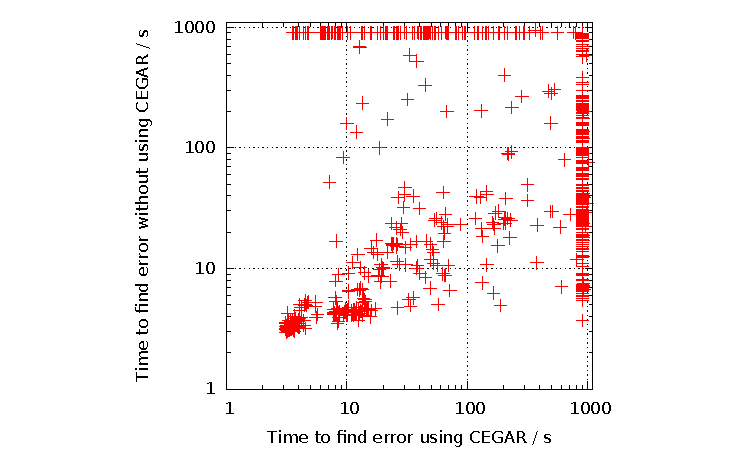
\includegraphics[trim=2cm 0 1cm 0, clip=true, scale=.9]{evaluation/sp_timeToFindError_cegar_noCegar}
\caption{Time in seconds to find an error}
\label{fig:spTimeToFindError}
\end{subfigure}%
\hfill
\begin{subfigure}[b]{.48\textwidth}
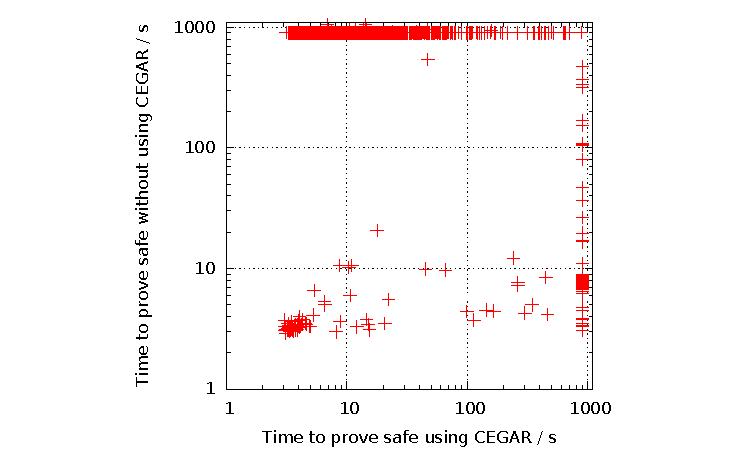
\includegraphics[trim=2cm 0 1cm 0, clip=true, scale=.9]{evaluation/sp_timeToProveTrue_cegar_noCegar}
\caption{Time in seconds to prove a program safe}
\label{fig:spTimeToProveSafe}
\end{subfigure}
\caption{Runtime performance of symbolic execution with and without CEGAR in comparison}
\end{figure}

Most of the programs with these characteristics are of the task sets of ProductLines and ECA.
To recap, of the 598~tasks symbolic execution without CEGAR can correctly find errors in, more than half (323~tasks) can't be analysed correctly by symbolic execution with CEGAR
due to many infeasible error paths and the resulting amount of refinements.
On the other hand, symbolic execution with CEGAR is able to prove for 101~new tasks that an error exists in them.
This shows that the efficiency of symbolic execution with and without CEGAR strongly depends on the task on hand, especially when the program is not error-free.
Fig.~\ref{fig:spTimeToFindError} illustrates that for many programs, either symbolic execution with or without CEGAR is able to find a (possibly non-existent) error within 900~seconds, but not both.
For proving the safety of a program, analysis with CEGAR performs significantly better, being able to correctly analyse 1623~tasks more than analysis without CEGAR, but its laziness results in bad performance for some programs, too (Fig.~\ref{fig:spTimeToProveSafe}).

\begin{figure}[h!]
\centering
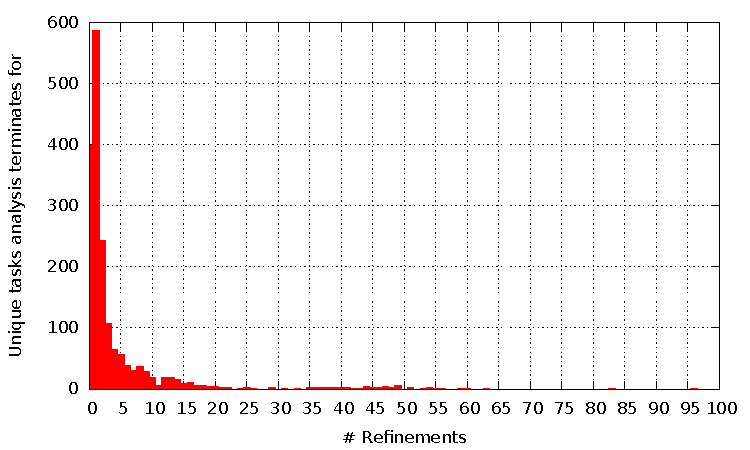
\includegraphics{evaluation/hg_refinementsForUniqueCorrects}
\caption{Amount of tasks analysis with CEGAR can compute a result for while analysis without CEGAR can't, and the number of refinements necessary for them}
\label{fig:hgRefinementsForUniques}
\end{figure}
\begin{figure}[h!]
\centering
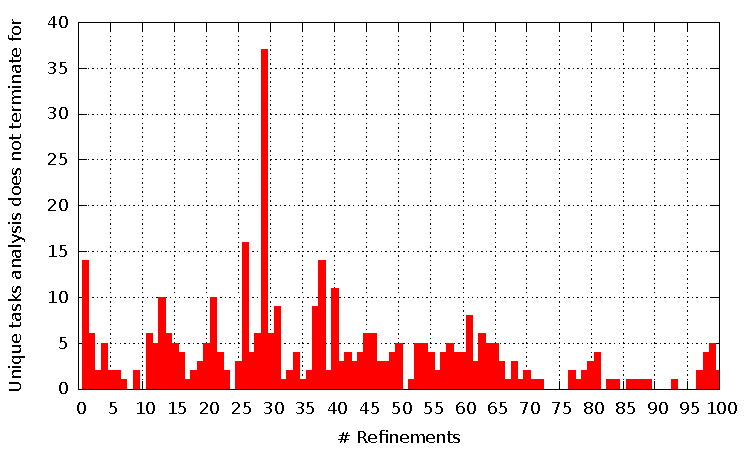
\includegraphics{evaluation/hg_refinementsForUniqueTimeouts}
\caption{Amount of refinements (up to 100) that were performed for a specific amount of tasks that resulted in a timeout}
\label{fig:hgRefinementsForTimeouts}
\end{figure}
For most tasks symbolic execution with CEGAR is able to compute a result but symbolic execution without CEGAR is not, only few or zero~refinements are necessary (Fig.~\ref{fig:hgRefinementsForUniques}).
Comparison with the random distribution of performed refinements in tasks that resulted in a timeout when using CEGAR (Fig.~\ref{fig:hgRefinementsForTimeouts}) confirms the problem CEGAR has with many possible error paths.

Nevertheless, thanks to its significant better performance in proving the safety of programs, CEGAR was able to push the \symbolicExecutionCPA's score from 660~points to 3271~points by increasing the amount of successfully verified
error-free tasks by more than~1500.

\subsection{Interpolation Techniques}
\label{sec:eval:itpTechniques}
\begin{table}[t]
\centering
\begin{tabular}{|r|c|c|c|c|}
\hline
                               & Values only & Values first & Constraints first & Overall \\ \hline
correct results                & 2080        & 2079         & 2078              & 4092 \\ \hline
\resultFalse, correct          & 378         & 376          & 376               & 2911 \\ \hline
\resultTrue, correct           & 1702        & 1703         & 1702              & 1181 \\ \hline
unique \resultFalse, correct   & 2           & 0            & 0                 & \\ \hline
unique \resultTrue, correct    & 0           & 0            & 0                 & \\ \hline
\resultFalse, incorrect        & 83          & 83           & 83                & \\ \hline
unique \resultFalse, incorrect & 0           & 0            & 0                 & \\ \hline
\resultTrue, incorrect         & 1           & 1            & 1                 & \\ \hline
unique \resultTrue, incorrect  & 0           & 0            & 0                 & \\ \hline
program errors                 & 3           & 3            & 2                 & \\ \hline % exception because of / 0, parsing error
%timeouts & 3275 & 1927 & \\ \hline
resource errors                & 1925        & 1926         & 1928              &\\ \hline % includes timeouts + StackOverflowException
\end{tabular}
\caption{Results of benchmark runs of the \symbolicExecutionCPA\ with CEGAR using three different techniques for interpolation computation}
\label{tab:itpTechniqueComp}
\end{table}
We compare three different techniques for computing interpolants of the \symbolicExecutionCPA\ already mentioned in Section~\ref{sec:assignmentRefinement}:
\begin{enumerate}[label=\alph*)]
\item Only removing unnecessary values and using all constraints that resulted from the previous interpolant and the strongest-post operator at the current edge (\emph{values only}),
\item removing unnecessary values first and then constraints (\emph{values first}), and
\item removing unnecessary constraints first and then values (\emph{constraints first}).
\end{enumerate}
Table~\ref{tab:itpTechniqueComp} shows that almost no difference exists in the effectivenes of all three techniques.
General time performance also differs in no significant way, as the scatter plots in Figure~\ref{fig:spTimeVOVF} show.
\begin{figure}[t]
\begin{subfigure}[b]{.48\textwidth}
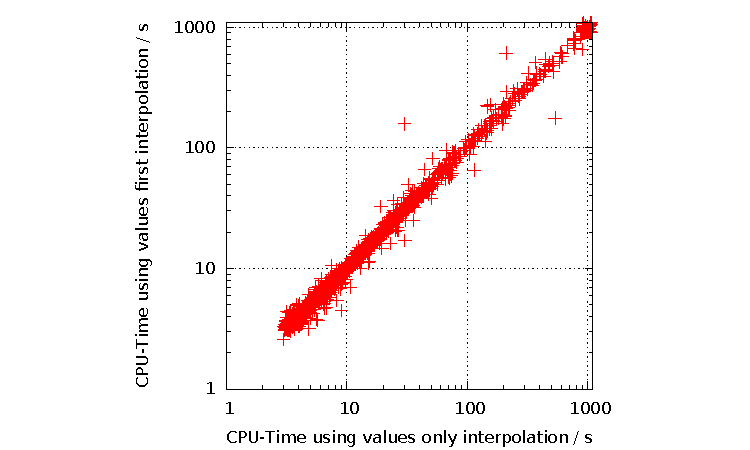
\includegraphics[trim=2cm 0 1cm 0, clip=true, scale=.9]{evaluation/sp_valuesOnly_valuesFirst_cputime}
\end{subfigure}%
\hfill
\begin{subfigure}[b]{.48\textwidth}
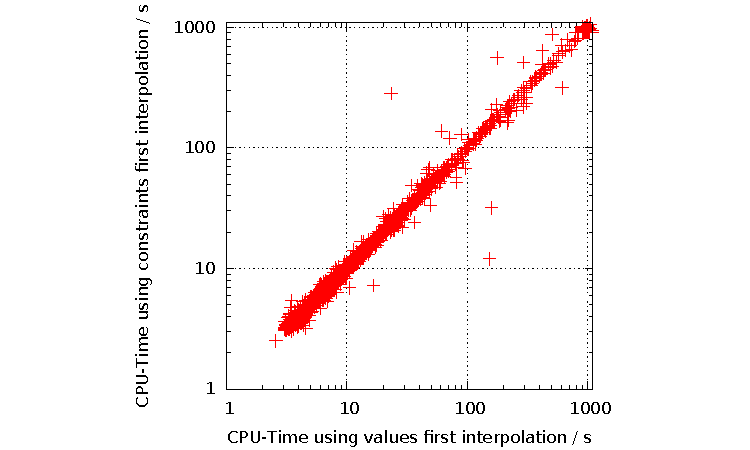
\includegraphics[trim=2cm 0 1cm 0, clip=true, scale=.9]{evaluation/sp_valuesFirst_constrFirst_cputime}
\end{subfigure}
\caption{Runtime performance of different interpolation techniques over all benchmark tasks}
\label{fig:spTimeVOVF}
\end{figure}
Using the values only interpolation technique yields two more correctly found errors over all benchmark tasks.
Both tasks are close to the time limit with 863.4 and 887.5 seconds.
The successful analysis of these two tasks is a result of the faster ''values only'' interpolant computation.
Since the strongest-post operator of symbolic execution refinement uses expensive SAT checks to check the satisfiability of current constraints, the two refinement procedures
''values first'' and ''constraints first'' take longer for a single refinement, as they call the strongest-post operator more often - for every abstract variable assignment and every constraint once, respectively.
The ''values only'' computation only calls the strongest-post operator once for every value, in contrast.
Similiarly, analyses using ''values only'' and ''values first'' are able to prove one more task safe then ''constraints first''.
This one is very close to the time limit (867.7 seconds using ''values only'', 836.6 seconds using ''values first''), too.

Analysis with interpolation using ''values first'' or ''constraints first'' is also able to prove one task safe ''values only'' can't.
Here, the computation times of 656.0 and 642.0 seconds are farther away from the time limit.
Although refinement takes longer then with ''values only'', the coarser precision of the \constraintsCPA\ speeds up termination of the analysis after all information necessary for proving all error paths are tracked.

For further evaluation we will use the ''constraints first'' technique, as it is the closest to our specification and does not pose any disadvantages in comparison to the other two techniques.

\subsection{Precision Types}

\begin{table}[t]
\centering
\begin{tabular}{|r|c|c|c|c|}
\hline
                               & Constraint & Location & Overall \\ \hline
correct results                & 2078       & 2083     & 4092 \\ \hline
\resultFalse, correct          & 376        & 384      & 2911 \\ \hline
\resultTrue, correct           & 1702       & 1699     & 1181 \\ \hline
unique \resultFalse, correct   & 1          & 3        & \\ \hline
unique \resultTrue, correct    & 6          & 9        & \\ \hline
\resultFalse, incorrect        & 83         & 83       & \\ \hline
unique \resultFalse, incorrect & 0          & 0        & \\ \hline
\resultTrue, incorrect         & 1          & 1        & \\ \hline
unique \resultTrue, incorrect  & 0          & 0        & \\ \hline
program errors                 & 2          & 2        & \\ \hline % exception because of / 0, parsing error
%timeouts & 3275 & 1927 & \\ \hline
resource errors                & 1928       & 1923     &\\ \hline % includes timeouts + StackOverflowException
\end{tabular}
\caption{Results of benchmark runs of the \symbolicExecutionCPA\ with CEGAR using constraints-based and location-based precision for \constraintsCPA}
\label{tab:precType}
\end{table}

\begin{figure}
\begin{subfigure}[b]{.48\textwidth}
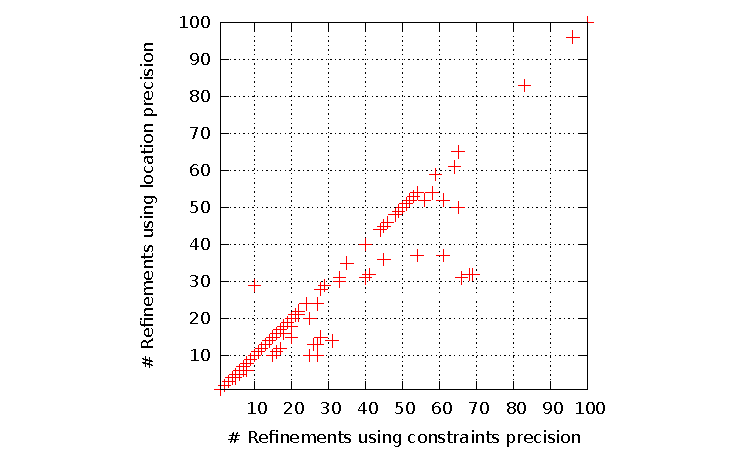
\includegraphics[trim=2cm 0 1cm 0, clip=true, scale=.9]{evaluation/sp_constPrec_locPrec_refinementsErrorFinding}
\caption{For finding an error}
\label{fig:precType:refsFalse}
\end{subfigure}%
\hfill
\begin{subfigure}[b]{.48\textwidth}
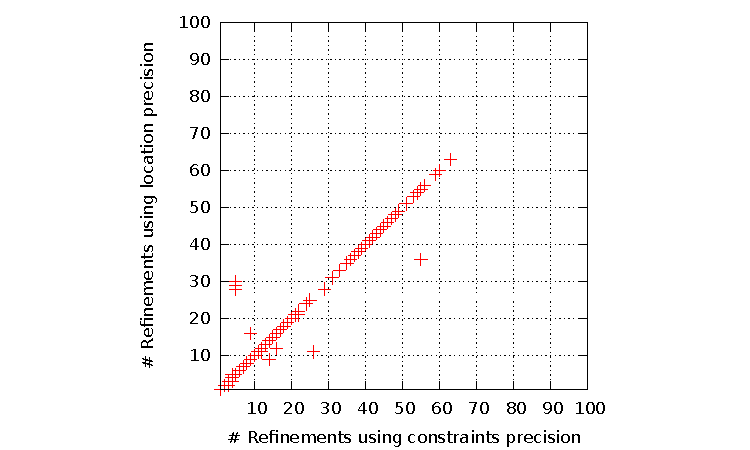
\includegraphics[trim=2cm 0 1cm 0, clip=true, scale=.9]{evaluation/sp_constPrec_locPrec_refinementsSafeProving}
\caption{For proving a program safe}
\label{fig:precType:refsTrue}
\end{subfigure}
\caption{Number of needed refinements for finding errors and proving a program safe}
\end{figure}

Table~\ref{tab:precType} shows the performance of the \symbolicExecutionCPA with CEGAR using the default constraints-based precision in comparison to the location-based precision.
As it is already the case with the ''value only'' interpolation technique, using the location-based precision provides a small boost in the amount of correctly found property violations in exchange for a small decrease in tasks correctly proven safe.
This is due to less needed refinements to reach a necessary precision to either find a feasible error path (Fig.~\ref{fig:precType:refsFalse}) or prove a program safe (Fig.~\ref{fig:precType:refsTrue}), as more constraints are tracked potentially.
To prove a program safe, only few variables and constraints have to be tracked, most of the time, though.
Because of this, the higher precision and the resulting bigger state space is often hindering when proving the safety of a program.

\subsection{Less-or-equal Operators}
\begin{table}[t]
\centering
\begin{tabular}{|r|c|c|c|c|}
\hline
                               & Subset        & Implication & Overall \\ \hline
correct results                & 2078       & 2078     & 4092 \\ \hline
\resultFalse, correct          & 376        & 376     & 2911 \\ \hline
\resultTrue, correct           & 1702       & 1702    & 1181 \\ \hline
unique \resultFalse, correct   & 1          & 1     & \\ \hline
unique \resultTrue, correct    & 0          & 0         & \\ \hline
\resultFalse, incorrect        & 83         & 83  & \\ \hline
unique \resultFalse, incorrect & 0          & 0            & \\ \hline
\resultTrue, incorrect         & 1          & 1            & \\ \hline
unique \resultTrue, incorrect  & 0          & 0            & \\ \hline
program errors                 & 2          & 2              & \\ \hline % exception because of / 0, parsing error
%timeouts & 3275 & 1927 & \\ \hline
resource errors                & 1928       & 1928      &\\ \hline % includes timeouts + StackOverflowException
\end{tabular}
\caption{Results of benchmarks runs of the \symbolicExecutionCPA\ with CEGAR using the subset and the implication less-or-equal operator with the constraints-based precision for the \constraintsCPA}
\label{tab:leqOp}
\end{table}

\begin{table}[t]
\centering
\begin{tabular}{|r|c|c|c|c|}
\hline
                               & SL         & IL       & Overall \\ \hline
correct results                & 2083       & 2079     & 4092 \\ \hline
\resultFalse, correct          & 384        & 384      & 2911 \\ \hline
\resultTrue, correct           & 1699       & 1695     & 1181 \\ \hline
unique \resultFalse, correct   & 1          & 1        & \\ \hline
unique \resultTrue, correct    & 4          & 0        & \\ \hline
\resultFalse, incorrect        & 83         & 83       & \\ \hline
unique \resultFalse, incorrect & 0          & 0        & \\ \hline
\resultTrue, incorrect         & 1          & 1        & \\ \hline
unique \resultTrue, incorrect  & 0          & 0        & \\ \hline
program errors                 & 2          & 3        & \\ \hline % exception because of / 0, parsing error
%timeouts & 3275 & 1927 & \\ \hline
resource errors                & 1923       & 1926     &\\ \hline % includes timeouts + StackOverflowException
\end{tabular}
\caption{Results of benchmark runs of the \symbolicExecutionCPA\ with CEGAR using subset (SL) and implication (IL) less-or-equal operator with the location-based precision for \constraintsCPA}
\label{tab:leqOpOnLocPrec}
\end{table}

The implication less-or-equal operator never performs better than the subset less-or-equal operator when using the constraints-based precision for the \constraintsCPA\ and worse than the subset less-or-equal operator when using the location-based precision. Tables~\ref{tab:leqOp} and~\ref{tab:leqOpOnLocPrec} show the results for benchmarks using these two different less-or-equal operators.
The reason for this is the fixedness of constraints:
The possibility that a state using a subset of or the same symbolic identifiers than another state consists of constraints that are implied by the other state without being a subset of its constraints, is very low.
Figure~\ref{fig:leqComp:stopAmount} illustrates that this is the case very seldomly.

\begin{figure}
\begin{subfigure}{.48\linewidth}
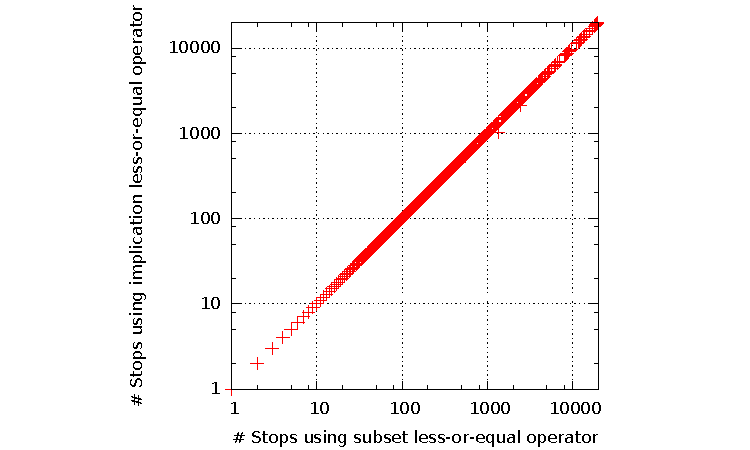
\includegraphics[trim=2cm 0 1cm 0, clip=true, scale=0.9]{evaluation/sp_leqSub_leqImpl_stops}
\caption{Using the constraint-based precision}
\end{subfigure}%
\hfill
\begin{subfigure}{.48\linewidth}
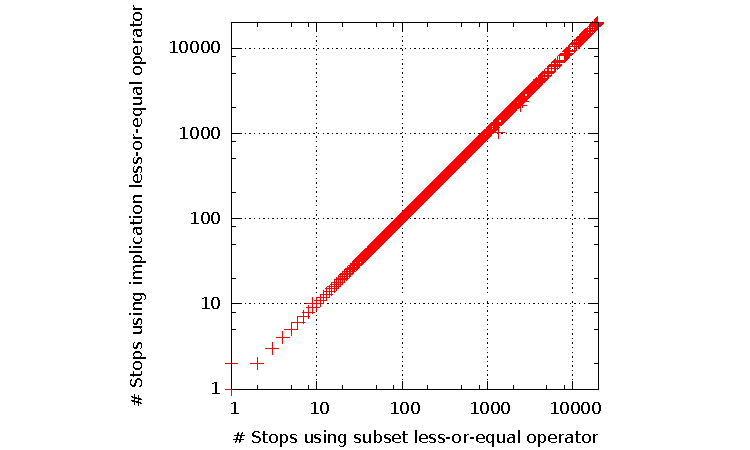
\includegraphics[trim=2cm 0 1cm 0, clip=true, scale=0.9]{evaluation/sp_leqSub_leqImpl_stopsLocPrec}
\caption{Using the location-based precision}
\end{subfigure}
\caption{Number of times stopped with subset and implication less-or-equal operator}
\label{fig:leqComp:stopAmount}
\end{figure}


\subsection{Sliced Prefix Selection}
The use of sliced prefix selection \cite{Beyer2015} \cite{Beyer2015a} (Sec.~\ref{sec:assignmentRefinement}) is able to boost the performance of the \symbolicExecutionCPA\ with CEGAR significantly.
Table~\ref{tab:prefSel} shows the benchmark results of the following selected prefix selection preferences:
\begin{itemize}
\item Random prefix selection, used as reference selection preference.
\item Selection of the shortest prefix, \emph{length short}.
\item Selection of the prefix based on a score computed from the variable types, easy types like boolean and integer being preferred. (domain good, \emph{DG})
\item Selection of the prefix based on a score computed from the variable types equal to ''DG'', but mixed with a score based on the size of the interpolants, preferring smaller ones. (domain good, narrow, \emph{DGN})
\item Selection of the prefix containing the fewest assignments, \emph{AmF}.
\item Selection of the prefix containing the fewest assumptions, \emph{AtF}.
\item Selection of the prefix containing the most assumptions, \emph{AtM}.
\item Selection of the prefix closest to the initial location of the error path. (pivot shallow, \emph{PS})
\end{itemize}
For all preferences but the random one a second preference exists if multiple prefixes are equal in concern to the preference:
\emph{short} for choosing the shortest prefix with the best score and \emph{long} for choosing the longest prefix with the best score.
More information about the individual prefix preferences can be found in \cite{Beyer2015a}.

\begin{table}[t]
\centering
\begin{tabular}{|r|c|c|c|c|c|}
\hline
Pref.Selection & \resultFalse, corr. & \resultTrue, corr. & \resultFalse, incorr. & \resultTrue, incorr. & Score \\ \hline
Random         & 488 & 1806   &  88 & 1 & 3560 \\ \hline
Length short   & 454 & 1738   &  93 & 1 & 3366 \\ \hline
DG short       & 476 & \cellcolor{LightGreen} 2000   &  94 & 1 & \cellcolor{LightGreen} 3906 \\ \hline
DG long        & 466 & 1949   &  93 & 1 & 3800 \\ \hline 
DGN short     & 482 & 1988   &  93 & 1 & 3888 \\ \hline
AmF short      & 459 & 1688   &  82 & 1 & 3331 \\ \hline
AmF long       & 407 & 1691   &  84 & 1 & 3279 \\ \hline
AtF short      & 475 & \cellcolor{LightRed} 1624   &  93 & 1 & \cellcolor{LightRed} 3159 \\ \hline
AtF long       & 412 & 1672   &  82 & 1 & 3258 \\ \hline
AtM short      & \cellcolor{LightGreen} 522 & 1843   &  93 & 1 & 3638 \\ \hline
AtM long       & \cellcolor{LightRed} 391 & 1827   &  92 & 1 & 3487 \\ \hline
PS short       & 447 & 1812   &  94 & 1 & 3501 \\ \hline
PS long        & 516 & 1810   &  88 & 1 & 3602 \\ \hline
\end{tabular}
\caption{Benchmark results for different prefix selection types, best and worst results highlighted}
\label{tab:prefSel}
\end{table}

It is clearly visible that performance of analysis strongly depends on the type of interpolants used for refinement, with symbolic execution being able to prove the safety of 366~more tasks when using the prefix selection preference \emph{domain good, short} in contrast to \emph{assumptions fewest, short}.

Using preferences aiming at increasing precision fast like \emph{assumptions most, short} or \emph{pivot shallow, long} allows analysis to find more errors thanks to its faster-growing precision and fewer needed refinements, just as expected.
Preference \emph{assumptions most, short} increases the precision of the \constraintsCPA as fast as possible by always incrementing the amount of constraints tracked as much as possible by choosing sliced prefixes relying on the most assumptions for proving infeasibility of the prefix.
Preference \emph{pivot shallow, long}, chooses the prefixes closest to the initial location of the error path so that new precisions are propagated to the most abstract states possible. It takes the longest prefixes, in addition, so that precision grows fast.
Increasing precision fast and continuing analysis after refinement higher in the abstract reachability graph avoids unnecessary refinements for error paths that are infeasible for the same reasons.
An example CFA for this benefit can be seen in Fig.~\ref{fig:cfaBadPref}.
While it is similar to the CFA in Fig.~\ref{fig:cegarFailsEx:cfa}, expensive refinement procedures can be avoided by choosing to track program variable $var$.
If the prefix preference always chooses sliced prefixes close to the target location, three~refinement procedures are necessary at the end of which program variables $a$, $b$ and $c$ are tracked.
If the prefix preference chooses the sliced prefix using program variable $var$, analysis already terminates after one~refinement.

\begin{figure}[t]
\centering
\begin{tikzpicture}[->,>=stealth, mynode/.style={circle, draw, minimum size=0.5cm}, every node/.style={font=\small}]

\node[mynode] (-1) {0};
\node[mynode] (-2) [below = 0.6cm of -1] {1};
\node[mynode] (l-3) [below left = 0.5cm and 0.8cm of -2] {2};
\node[mynode] (0) [below right = 0.7cm and 0.8cm of -2]{3};
\node[mynode] (1) [below = 0.6cm of 0] {4};
\node[mynode] (l2) [below left = 0.7cm and 0.8cm of 1] {5};
\node[mynode] (r2) [below right = 0.7cm and 0.8cm of 1, draw=red, very thick] {6};
\node[mynode] (ll3) [below left = 0.7cm and 0.6cm of l2] {7};
\node[mynode] (lr3) [below right = 0.7cm and 0.6cm of l2, draw=red, very thick] {8};
\node[mynode] (llr4) [below right = 0.7cm and 0.4cm of ll3, draw=red, very thick] {9};
\node[mynode] (lll4) [below left = 0.7cm and 0.4cm of ll3] {10};

\path
  (-1) edge node [left] {\textbf{var $\assign$ 2}} (-2)
  (-2) edge node [left] {$\mathbf{[var == 2]}$} (l-3)
  (-2) edge node [right] {$\mathbf{[!(var == 2)]}$} (0)
  (0) edge node [left] {\textbf{a $\assign$ 2, b $\assign$ 2, c $\assign$ 2}} (1)
  (1) edge node [left, pos=0.3] {$\mathbf{[!(a == 1)]}$} (l2)
  (1) edge node [right, pos=0.3] {$\mathbf{[a == 1]}$} (r2)
  (l2) edge node [left, pos=0.3] {$\mathbf{[!(b == 1)]}$} (ll3)
  (l2) edge node [right, pos=0.3] {$\mathbf{[b == 1]}$} (lr3)
  (ll3) edge node [right, pos=0.3] {$\mathbf{[c == 1]}$} (llr4)
  (ll3) edge node [left, pos=0.3] {$\mathbf{[!(c == 1)}$} (lll4)
;
\end{tikzpicture}
\caption{CFA representing a program that creates problems when using the wrong prefix selection preference}
\label{fig:cfaBadPref}
\end{figure}

In contrast to these, \emph{assumptions fewest, short} has the slowest growing precision, increasing precision of the \constraintsCPA\ only as little as possible by choosing the fewest assumptions possible and precision of the \symbolicValueAnalysisCPA\ only as much as needed to keep \constraintsCPA's precision low by choosing short prefixes.
The slow growth of precision is also the cause \emph{domain good, short} only performs mediocre in relation to the other analysis in finding errors.
Thanks to choosing variables whose types are easily handable by both the \valueAnalysisCPA\ and the \constraintsCPA, it boosts proving the safety of programs immensely.
For the domain-good preference, a more precise alternative exists. It performed worse then the default for all variations, though.

%The choice of long or complicated prefixes increases time for refinement, too.

It must be added that the benchmarks for sliced prefix preferences were run with configuration option \configOption{cpa.value.optimizeBooleanVariables=true}, which causes a bug for few tasks in the \symbolicExecutionCPA.
When using \emph{domain good, short}, one task was affected by this error, which exceeds the time limit with the option turned off.
For \emph{assumptions fewest, short} and \emph{pivot shallow, long}, no task was affected.
For \emph{assumptions most, short}, 5 tasks were affected. It still is the best preference for finding errors and the fourth-best for proving the safety of programs.
Unfortunately there was no time to repeat all benchmarks with this option turned off due to their long runtime.

\subsection{Delegation to Concrete Value-Analysis Refinement}

\begin{table}[t]
\centering
\begin{tabular}{|r|c|c|c|}
\hline
                               & No delegation & Delegation  & Overall \\ \hline
correct results                & 2078       & 2081     & 4092 \\ \hline
\resultFalse, correct          & 376        & 423      & 2911 \\ \hline
\resultTrue, correct           & 1702       & 1658     & 1181 \\ \hline
unique \resultFalse, correct   & 64         & 20       & \\ \hline
unique \resultTrue, correct    & 86         & 89       & \\ \hline
\resultFalse, incorrect        & 83         & 84       & \\ \hline
unique \resultFalse, incorrect & 2          & 2        & \\ \hline
\resultTrue, incorrect         & 1          & 1        & \\ \hline
unique \resultTrue, incorrect  & 0          & 0        & \\ \hline
program errors                 & 2          & 3        & \\ \hline % exception because of / 0, parsing error
%timeouts & 3275 & 1927 & \\ \hline
resource errors                & 1928       & 1924     &\\ \hline % includes timeouts + StackOverflowException
\end{tabular}
\caption{Results of benchmark runs of the \symbolicExecutionCPA\ with CEGAR using no delegation (the default) and using delegation to concrete value-analysis only refinement, both using no prefix selection}
\label{tab:delegation}
\end{table}

Table~\ref{tab:delegation} shows the difference between analysis using CEGAR without and with delegation to refinement using concrete values only.
While sometimes analysis always using symbolic refinement (using no delegation) performs better and sometimes analysis performing concrete value analysis whenever possible performs better, 137~of the 184~differences appears in the ECA task set, where the kind of refinement is very important.

Although both techniques differ slightly in the tasks they can solve, delegation provides a significant boost to speed for tasks they can solve both (which are almost all of the tasks they can solve, after all).
Figure~\ref{fig:delegCputime} shows the CPU-time both analysis with CEGAR using no delegation and analysis with CEGAR using delegation claim for tasks they both terminate for with the same result (no matter whether it is correct or incorrect).
While there are some tasks analysis with delegation can solve faster using symbolic refinement all the time, it is clearly visible that for the majority of tasks, analysis using delegation performs significantly better.
This is attributed to the faster refinement procedure that goes without expensive SAT checks, in contrast to symbolic refinement.
Figure~\ref{fig:delegRefinetime} illustrates this difference in speed.

\begin{figure}
\centering
\begin{subfigure}[b]{.48\textwidth}
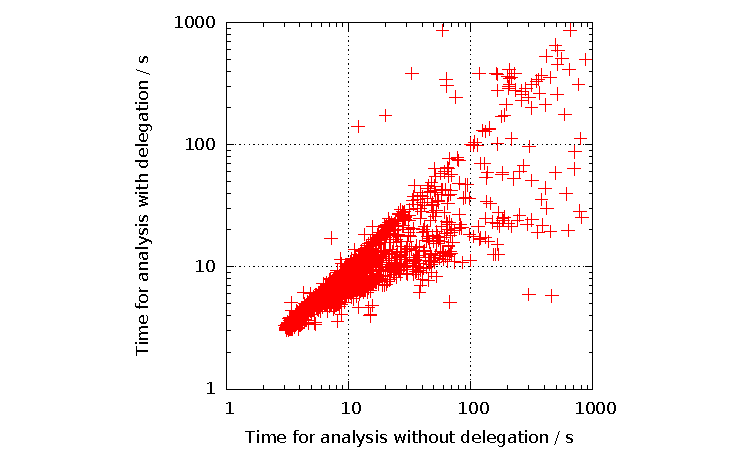
\includegraphics[trim=2cm 0 1cm 0, clip=true, scale=0.9]{evaluation/sp_cputime_noDeleg_deleg}
\caption{CPU-time for complete analysis}
\label{fig:delegCputime}
\end{subfigure}
\begin{subfigure}[b]{.48\textwidth}
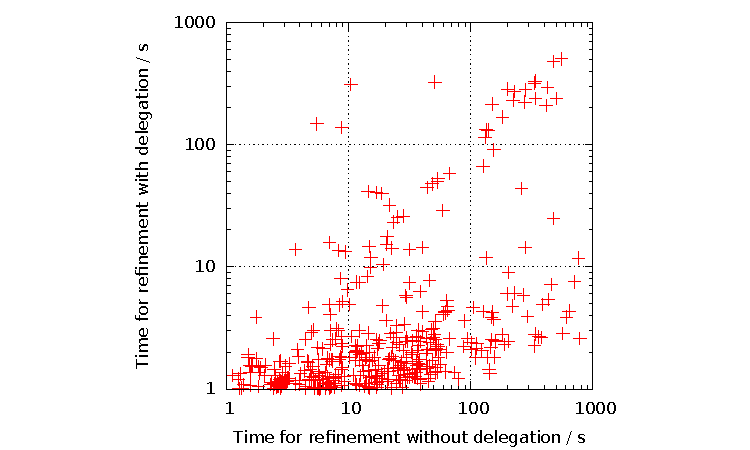
\includegraphics[trim=2cm 0 1cm 0, clip=true, scale=0.9]{evaluation/sp_refinetime_noDeleg_deleg}
\caption{CPU-time for refinement procedure}
\label{fig:delegRefinetime}
\end{subfigure}
\caption{Performance of analysis using CEGAR without delegation and with delegation for tasks both techniques terminate for with the same result}
\end{figure}
